\documentclass[aps,pre,preprint]{revtex4}
% \documentclass[aps,pre,twocolumn]{revtex4}
% \documentclass[aps,jcp,groupedaddress,twocolumn,unsortedaddress]{revtex4}

\usepackage{amsmath}
\usepackage{amssymb}
\usepackage[dvips]{graphicx}
\usepackage{color}
\usepackage{tabularx}

\makeatletter
\makeatother

\newcommand{\recheck}[1]{{\color{red} #1}}
\renewcommand{\v}[1]{\textbf{\textit{#1}}}
\renewcommand{\d}[1]{\textsf{#1}}


\begin{document}

\title{The Error Estimate of Force Calculation in the Heterogeneous Molecular Systems}
\author{Han Wang}
\affiliation{LMAM and School of Mathematical
  Sciences, Peking University}
\author{Pingwen Zhang}
% \email{pzhang@pku.edu.cn}
\affiliation{LMAM and School of Mathematical
  Sciences, Peking University}

\begin{abstract}
\end{abstract}

\maketitle

\section{Introduction}
Non-bonded short-range interaction is encountered in nearly every
molecular simulation.  A naive idea to calculate short-range
interactions is to explicitly calculate all pairwise
interactions. This results in a computational cost scaling $\mathcal
O(N^2)$ per time step, which rapidly becomes inefficient as the number
of particles $N$ grows large. A better way is to introduce a cut-off
radius, outside of which all pairwise interactions are simply
neglected. In combination with the cell list and the neighbor list
algorithms \cite{frenkel02b}, the total computational cost of the
short-range interactions can be reduced to an acceptable level of
$\mathcal O(N)$. The cut-off radius is only a user provided
algorithmetic parameter, so it should have no effect on the
physical/chemical properties of the system.  Therefore, it is very
important to test the convergence of the simulation results with
respect to the used cut-off radius before collecting data and deriving
conclusions. Fortunately, in most homogeneous systems, a satisfactory
convergence can be achieved even with a very small cut-off value, for
example, $2.5$ -- $4.0\sigma$.  Moreover, it is possible to correct
the systematic error of the potential energy, the pressure and the
free energy by applying the standard long range correction
(LRC)~\cite{allen87a}, which assumes the uniformity outside the
cut-off and integrates the contribution of the mentioned properties to
infinity.  However,
% The spacial inhomogenety of the system in terms of particle density,
% particle type and change distribution is very common in natrual
% system.
the direct molecular simulation of a inhomogeneous system will
encounter non-trival difficulty that does not exist in the homogeneous
bulk simulations.  The measured properties are found to depend on the
cut-off radius even at a very large value~\cite{duque2004some}. Also
the contiuity at the cut-off and the long-range correction involved
may have foundamental effect on the simulation
results~\cite{trokhymchuk1999computer, shen2007comparative,
  guo1997long, mecke1997molecular, janecek2006long, goujon2004monte}.
Therefore, it is necessary to systemetically study the precision of
short-range interaction calculation, and to develop methods screening
out the aforementioned cut-off artifect in the inhomogeneous systems.

% In this paper, we focus on the systems in which
% atoms/particles are interacting via short-range interactions, because
% it is a good starting point of the study of more complex systems, for
% example, the systems with long-range electrostatic interactions.  The
% simulation results in the inhomogeneous systems are found to depend on
% a number of factors of treating the short-range interaction in the
% simulation. For example, the way of calculating the short-range
% interaction (simple cut-off method or Ewald
% summation)~\cite{karasawa1989acceleration, lopez2002thermodynamic,
%   lopez2006liquid, shi2006molecular, ismail2007application}, the
% cut-off radius~\cite{trokhymchuk1999computer, duque2004some,
%   shen2007comparative}, the way of long-range
% correction~\cite{guo1997long, mecke1997molecular, janecek2006long,
%   goujon2004monte} and the size and shape of the simulation
% box~\cite{chen1995area, orea2005oscillatory, biscay2009calculation}.
% It should be noticed that the physical properties are the nature of
% the system, and should NOT depend on the details of the interaction
% calculation.


A promising way to quantitatively analyze the undesirable cut-off
effects is to express these artifacts in terms of the difference
between the cut-offed interaction and the exact interaction, namely
the error. In homogeneous systems, the error analysis of the
short-range interaction has been well established,
see~\cite{kolafa1992cutoff} for example. Also the error
estimates~\cite{hummer1995numerical, kolafa1992cutoff,
  petersen1995accuracy, deserno1998mue2, wang2010optimizing} for
long-range Ewald family methods~\cite{ewald1921die,
  hockney1988computer, deserno1998mue1, darden1993pme, essmann1995spm}
have provided a profound view of the precision of force calculation,
and introduced parameter tuning algorithms~\cite{limbach06a,
  wang2010optimizing} that boost the efficiency of the computation
with a good control of the error. However, in inhomogeneous systems
the error study is still scarce, even for the simplest short-range
interaction.

In this work, we develop the error estimate of the short-range force
in inhomogeneous systems. The force error can be split into the
homogeneous and inhomogeneous part regardless the correlation in the
system. The inhomogeneous error that can be more than one order of
maganitude larger than the homogeneous error plays a dominant role in
the interfacial region. An adaptive cut-off method is hereby proposed
to equally distribte the error according to the error estimate, so
that a substantial computational effort can be saved while the
precision of simulation is preserved. We also proposed a long-range
force correction method based on the error estimate to screen out the
contribution of the inhomogeneous error, which can tremendously
improve the precision of simulation. To show the effectiveness of the
error estimate and the proposed methods, two systems are tested: the
liquid-vapor equilibrium for equilibrium properties, and the colliding
nanoscale clusters for dynamical properties. Finally, a conclusion is
given in section \ref{sec:conclusion}.

% The error estimate of long-range algorithms, for example the Ewald
% family method~\cite{ewald1921die, hockney1988computer,
%   deserno1998mue1, darden1993pme, essmann1995spm} and the fast
% multipole method~\cite{greengard1987fast}, has been well developped in
% the past 20 years ~\cite{hummer1995numerical, kolafa1992cutoff,
%   petersen1995accuracy, deserno1998mue2, wang2010optimizing,
%   dachsel2009error}. 



\section{Theoretical background}
\subsection{Error estimate in a heterogeneous system}

Suppose the system is composed by $N$ identical particles located at
$\v r_1, \v r_2, \cdots, \v r_N$ with periodic boundary condition.
Since the error estimate developed for the one-component system can be
directly extended to multi-component system without substantial
difficulty, the discussion in this paper will focus on one-component
system for symplicity.  These particles are interacting via a
short-range pairwise interaction denoted by $u(\v r)$ and correspond
force denoted by $\v f(\v r)$, with a cut-off radius $r_c > 0$.  This
means the interaction between any pair of particles falling out of the
cut-off radius is neglected.  An infinite cut-off radius will lead to
a precise calculation of interaction, but it is impractical.  The
error of computing interaction is mainly introduced by a finit value
of the cut-off radius. For convenience, the complementary of the
cut-offed short-range force is defined by
\begin{align}
  \v f^c(\v r) =
  \left\{
  \begin{array}{ll}
    0, & \vert\v r\vert\leq r_c; \\
    \v f(\v r), & \vert\v r\vert > r_c.
  \end{array}
  \right.
\end{align}
To measure the error of force computing, we add a testing particle at
position $\v r$. The exact force and the computed force (or cut-offed
force) exerted by the system on the testing particle are denoted by
${\v F}(\v r)$ and $\tilde{\v F}(\v r)$, respectively.  The difference
between them, namely the \emph{error force}, is denoted by $\Delta\v
F(\v r) = \v F(\v r) - \tilde{\v F}(\v r)$, which can be expressed by
\begin{align}
  \Delta\v F(\v r) = \sum_{\v n}\sum_{j}\, \v f^c(\v r - \v r_j + \v n).
\end{align}
Where $\v n$ is simulation box vector, so the summation over $\v n$
indicates that all periodic images are consider in the force
calculation. In a homogeneous system with periodic boundary condition
applied, the surounding of any particle is isotropic, so the
\emph{mean error force} vanishes, namely $\langle\Delta\v F(\v
r)\rangle = 0$. However, in a heterogenous system, the mean error
force is not necessarily zero but
\begin{align} \label{eqn:tmp3} %\nonumber
  \langle\Delta\v F(\v r)\rangle
  &=
  \big\langle
  \sum_{\v n}\sum_{j}\, \v f^c(\v r - \v r_j + \v n)
  \big\rangle 
  =
  \int_{\mathbb R^3}\v f^c(\v r - \v r')\rho(\v r')\,\d d\v r'
\end{align}
Where $\rho(\v r)$ denotes the particle number density at the position
$\v r$, and is periodically extended to $\mathbb R^3$. And notice the
error force implicitly depends on the cut-off radius used for the
interaction.

The widely accepted definition of the force error is the \emph{root mean
square} (RMS) \emph{error}, namely the square root of the second moment of the
error force is $\mathcal E(\v r) = \sqrt{\langle\vert\Delta\v F(\v
  r)\vert^2\rangle}$, which can be calculate by
\begin{align} \nonumber
  \langle\vert\Delta\v F(\v r)\vert^2\rangle
  =\,&
  \big\langle\sum_{j,k}\v f^c(\v r - \v r_j)\cdot\v f^c(\v r - \v r_k)\big\rangle \\ \nonumber
  =\,&
  \big\langle\sum_j\vert\v f^c(\v r - \v r_j)\vert^2\big\rangle +
  \big\langle\sum_{j\neq k}\v f^c(\v r - \v r_j)\cdot\v f^c(\v r - \v r_k)\big\rangle \\ \nonumber
  =\,&
  \int_{\mathbb R^3}\vert\v F^c(\v r - \v r')\vert^2\rho(\v r')\,\d d\v r'
  + \\\label{eqn:tmp4}
  \,&
  \int_{\mathbb R^3\times\mathbb R^3}\v F^c(\v r - \v r')\cdot\v F^c(\v r - \v r'')\rho(\v r', \v r'')\,\d d\v r'\d d\v r'',
\end{align}
The density $\rho(\v r')$ and the pair density $\rho(\v r', \v r'')$
are related to the probability density $p(\v r')$ and pair probability
density $p(\v r', \v r'')$ by
\begin{align}
  \rho(\v r') &= N\,p(\v r') \\
  \rho(\v r', \v r'') &= N(N-1)\,p(\v r', \v r'')
\end{align}
The pair density is also periodically extented to the whole space $\mathbb
R^3$.
% The problem now this how to discretize the integrals in
% \eqref{eqn:tmp4}. With the piecewise constant numerical integration
% formulus, we have:
Now, let
\begin{align} \nonumber
  \rho(\v r', \v r'')
  & = N (N-1) \,p(\v r', \v r'') \\\nonumber
  & = N (N-1) \big\{ p(\v r')p(\v r'') + [\,p(\v r', \v r'') -  p(\v r')p(\v r'')\,]\big\} \\\nonumber
  &= \frac{N-1}N \rho(\v r')\rho(\v r'') + C (\v r', \v r'')\\ \label{eqn:tmp7}
  &\approx \rho(\v r')\rho(\v r'') + C (\v r', \v r'')
\end{align}
the function
\begin{align}
C (\v r', \v r'') = N (N-1) [\,p(\v r', \v r'') -  p(\v r')p(\v r'')\,]
\end{align}
denotes the correlation between
position $\v r'$ and $\v r''$. Therefore, \eqref{eqn:tmp4} becomes
\begin{align} \nonumber
  \langle\vert\Delta\v F(\v r)\vert^2\rangle
  = &\,
  \int_{\mathbb R^3}\vert\v f^c(\v r - \v r')\vert^2\rho(\v r')\,\d d\v r' \,+ \\\nonumber
  &\,
  \bigg[\int_{\mathbb R^3}\v f^c(\v r - \v r')\rho(\v r')\,\d d\v r'\,\bigg]^2 + \\\nonumber
  &\,
  \int_{\mathbb R^3\times\mathbb R^3}\v f^c(\v r - \v r')\cdot\v f^c(\v r - \v r'')\,C(\v r', \v r'')\,\d d\v r'\d d\v r'' \\\label{eqn:tmp5}
  = &\,
  \mathcal E_{\textrm{homo}}(\v r) +
%  \langle\Delta\v F(\v r)\,\rangle^2 +
  \mathcal E_{\textrm{hetero}}(\v r) +
  \mathcal E_{\textrm{correlation}}(\v r)
\end{align}
If the system is homogeneous and the correlation between particles is
neglected, then only the first term, which is called the homogeneity
error, is left in \eqref{eqn:tmp5}. This term is originated from the
flucuation of the error force $\Delta\v F(\v r)$. The second term is
called the heterogeneity error, because it generates due to the
density heterogeneity of the system. It is worth poining out that the
heterogeneity error is the nothing but the squared mean error force,
namely $\mathcal E_{\textrm{hetero}}(\v r) = \langle\Delta\v F(\v
r)\,\rangle^2$.  The last term in \eqref{eqn:tmp5} originates from the
correlation between the particles, so it is called the correlation
error.  The correlation error involves a double integral, which
implies that calculating this term requires more compuational cost
than the homogeneity and heterogeneity errors. The rest of this paper
assumes the system is far from the critical point, therefore the
correlation error does not dominate in the system, and can be savely
neglected.



\subsection{The fast calculation of the error estimate}\label{sec:tmp1.3}

The naive calculation of the error estimate \eqref{eqn:tmp5} requires
the compuational cost of $\mathcal O(N^2)$. To apply the error
estimate on-the-fly with simulation, the compuational cost should be
reduced to at least $\mathcal O(N\log N)$.  This is achieved by
calculating the convolutions in \eqref{eqn:tmp5} with the fast Fourier
transform. We assume the simulation box is uniformly divided in to
small bins.  The positions of these bins are
\begin{align}
  \v r_{i_1, i_2, i_3} & =
  \frac{i_1}{K_1}\v a_1 + 
  \frac{i_2}{K_2}\v a_2 + 
  \frac{i_3}{K_3}\v a_3,\qquad 0\leq i_\alpha< K_\alpha
\end{align}
where $\v a_\alpha$ are box vectors, and $K_\alpha$ is the number of
division on each direction. In the reciprocal space, a corresponding
lettice is set up:
\begin{align}
  \v k_{k_1, k_2, k_3} & =
  k_1\v a_1^\ast +
  k_2\v a_2^\ast +
  k_3\v a_3^\ast, \qquad 0\leq k_\alpha<K_\alpha
\end{align}
where $\v a_\alpha^\ast$ are reciprocal box vectors defined by $\v
a_\alpha\cdot\v a_\beta^\ast = \delta_{\alpha\beta}$.  In each bin the
error and the particles number density are assumed to be constant,
therefore,
\begin{align}\nonumber
  \mathcal E_{\textrm{homo}}(\v r_{i_1,i_2,i_3})
  & \approx
  \frac1V\sum_{k_1=-\infty}^\infty\sum_{k_2=-\infty}^\infty\sum_{k_3=-\infty}^\infty
  \hat{\mathcal E}_{\textrm{homo}}(\v k_{k_1,k_2,k_3})
  % e^{2\pi i\v k_{k_1,k_2,k_3}\cdot\v r_{i_1,i_2,i_3}}
  \exp\bigg[
  2\pi i\bigg(
  \frac{k_1i_1}{K_1} + \frac{k_2i_2}{K_2} + \frac{k_3i_3}{K_3}
  \bigg)
  \bigg] \\\label{eqn:tmp13}
  & \approx
  \frac1V\sum_{k_1=0}^{K_1}\sum_{k_2=0}^{K_2}\sum_{k_3=0}^{K_3}
  \hat{K}_{\textrm{homo}}(\v k'_{k_1,k_2,k_3})\:
  \hat{\rho}(\v k_{k_1,k_2,k_3})
  % e^{2\pi i\v k_{k_1,k_2,k_3}\cdot\v r_{i_1,i_2,i_3}}
  \exp\bigg[
  2\pi i\bigg(
  \frac{k_1i_1}{K_1} + \frac{k_2i_2}{K_2} + \frac{k_3i_3}{K_3}
  \bigg)
  \bigg]   
\end{align}
here we denote the convolution kernel $\vert\v f^c(\v r)\vert^2$ by
$K_{\textrm{homo}}(\v r)$.  Equation \eqref{eqn:tmp13} simply utilizes
the identity: the Fourier transform of the convolution
$K_{\textrm{homo}}\ast\rho$ is equal to the multiply of
$\hat{K}_{\textrm{homo}}$ and $\hat\rho$.  The prime on $\v
k_{k_1,k_2,k_3}$ means that we should use the periodic image $k_\alpha
- K_\alpha$ instead of $k_\alpha$ when $k_\alpha \geq K_\alpha/2$. By
definition, the Fourier transform of the density is
\begin{align}
  \hat\rho(\v k_{k_1,k_2,k_3})
  & \approx
  \frac{V}{K_1K_2K_3}
  \sum_{i_1=0}^{K_1}\sum_{i_2=0}^{K_2}\sum_{i_2=0}^{K_2}
  \rho(\v r_{i_1,i_2,i_3})
  \exp\bigg[
  -2\pi i\bigg(
  \frac{k_1i_1}{K_1} + \frac{k_2i_2}{K_2} + \frac{k_3i_3}{K_3}
  \bigg)
  \bigg]
\end{align}
The Fourier transform of the homogeneity kernel is 
\begin{align}
  \hat K_{\textrm{homo}}(\v k)
  &=
  \int_{\mathbb R^3}K_{\textrm{homo}}(\v r)e^{-2\pi i\v k\cdot\v r}\,\d d\v r
\end{align}
Most of the short-range interactions are isotropic, therefore,
$K_{\textrm{homo}}(\v r) = K_{\textrm{homo}}(r)$, and
\begin{align}
  \hat{K}_{\textrm{homo}}(\v k)
  =
  \int_{\mathbb R^3}K_{\textrm{homo}}(r)e^{-2\pi i\v k\cdot\v r}\d d\v r
  =
  \int_{r_c}^\infty \frac{2 r}k\, K_{\textrm{homo}}(r) \sin(2\pi kr)\,\d dr
\end{align}


Similarly, by \eqref{eqn:tmp3}, the Fourier mode of the the mean error
force is
\begin{align}\label{eqn:tmp17}
  \langle\Delta\v F\rangle^\wedge(\v k) =
  \hat{\v f}^c(\v k)\,
  \hat\rho(\v k)
\end{align}
where 
\begin{align}\label{eqn:tmp18}
  \hat{\v f}^c(\v k) 
  & = 
  2\pi\frac{\v k}k\, i\,
  \bigg\{
  r_c^2\,u(r_c)
  \bigg[\,
  \frac{2\cos(2\pi kr)}{2\pi kr}
  -\frac{2\sin(2\pi kr)}{(2\pi kr)^2}
  \,\bigg] 
  -
  \int_{r_c}^\infty 2r\,u(r)\sin(2\pi kr)\,\d d\v r
  \bigg\}
\end{align}


\subsection{The adaptive cut-off radius method}

% In Fig. \ref{fig:tmp1}, the testing system containing $N=16000$
% standard Lennard-Jone particles is set up in a tube with periodic
% boundary condition. The liquid droplet (in the middle of the tube) is
% in equilibrium with the surrounding vapor environment. The red line in
% the Fig. \ref{fig:tmp2} denotes the density profile (on direction $x$)
% of this heterogeneous system. The green square denotes the real RMS
% force error distribution. It is clear that the error form two peaks in
% the interfacial region, which is much higher than the relative
% constant error of the bulk liquid and the bulk vapor. The dashed and
% the dotted blue line are the estimated homogeneity and heterogeneity
% errors, and the solid blue line is the sum. In the bulk region, the
% homogeneity error dominates while in the interfacial region, the
% heterogeneity error dominates. The esitmated error matches perfactly
% with the real error at the interfacial region, but presents
% overestimation in the bulk regions. The overestimation probably stems
% from the neglection of the correlation error in \eqref{eqn:tmp5}.

A basic observation in a heterogeneous system is that the RMS force
error is not uniformly distributed. The difference between the maximum
and minimum error can be as large as two orders of maganitude, see
Fig. \ref{fig:tmp2}. Traditionally, a very large cut-off radius is
used to reduce the maximum error to an acceptable level and to reach
convergent simulation results. However, a huge amount of compuational
effort is wasted in the low-error region. The idea of the adaptive
cut-off radius simulation is to use larger cut-off radius for
particles in the high-error region to control the force error, while
to use smaller cut-off radius for particles in the low-error region to
save compuational cost.  The vaidity of this method relies on a
diliberated cut-off choice for each particle so that the force error
is uniformly distributed across the simulation region.  Unfortunately,
the compuational expense of a naive implementation of this method is
at least $\mathcal O(N^2\log N)$.  Becasue to determine the cut-off
radius, we should estimate the RMS force error at least once for each
particle, and the computational cost of each force error estimate is
$\mathcal O(N \log N)$.


% Since heterogeneity error dominate the
% force error of the system, such a big cutoff radius is a waste in the
% bulk liquid and vapor regions. One possible way is to use adapt
% cut-off radius according to the error distribution, so that larger
% cut-off radii are used in the interfacial region while smaller cut-off
% radii are used in the bulk regions.  More precisely, the aim of the
% adaptive cut-off method is to equivalently distributed the force error
% over the simulation region.

To make the adaptive cut-off method feasible,
\begin{enumerate}
\item The space is divided in to small bins, the size of which is the
  same as those mentioned in the section \ref{sec:tmp1.3}.  The
  particles falling in the same bin are assigned by the same cut-off
  radius.
  % The cut-off
  % radius is assumed to be constant within a bin, no matter the
  % position of the partile.
\item The cut-off radius can only be chosen from a discrete series of
  increasing values between a maximum cut-off radius
  $r_c^{\textrm{max}}$ and a minimum cut-off radius
  $r_c^{\textrm{min}}$: $\{\,r_c^{\textrm{min}} = r_c^0 < r_c^1 <
  \cdots < r_c^{M-1} <r_c^M = r_c^{\textrm{max}}\}$.  We call it the
  \emph{candidate set} of cut-off radii.  For convenience but not
  necessarily, the interval between two neighboring cut-off radius in
  uniform, which means
  \begin{align}
    r_c^m = r_c^0 + r_c^{\textrm{step}} m, \quad 0 \leq m \leq M
  \end{align}
  For example, a possible candidate set is $\{2.5\,\sigma,\
  3.0\,\sigma,\ 3.5\,\sigma,\ 4.0\,\sigma,\ \cdots,\ 10.0\,\sigma\}$,
  with $r_c^{\textrm{max}} = 10.0\sigma$, $r_c^{\textrm{min}} =
  2.5\sigma$ and $r_c^{\textrm{step}} = 0.5 \sigma$.
\end{enumerate}
For each cut-off radius in the candidate set, the force error
distribution $\mathcal E(\v r)$ is calculated by estimate
\eqref{eqn:tmp5}. Notice the error is calculated on-the-fly by the
fast algorithm described in section \ref{sec:tmp1.3}, therefore it is
defined on the bins.  For a predetermined error control level
$\mathcal E_{\textrm{C}}$, a satisfactory cut-off radius of a bin is
choosen such that it is the smallest one that satisfying the precision
constrain $\mathcal E(\v r_{i_1,i_2,i_3}) \leq \mathcal
E_{\textrm{C}}$. The computational cost of this algorithm is $\mathcal
O(MN\log N)$.  The idea of this algorithm is based on the observation
that the cut-off radius may not be calculated at a very high
precision, a slightly (and at most $r_c^{\textrm{step}}$) larger
cut-off radius will not waste too much computational cost.  Due to the
thermodynamic flucuation of the system density, the resulting cut-off
distribution $r_c(\v r_{i_1,i_2,i_3})$ (as a function of lattice
position) needs to be refined by the following scheme:
\begin{align}\label{eqn:rc-refine}
  r^{(1)}_c(\v r_{i_1,i_2,i_3}) = \max_{j_\alpha\in I}\,r_c(\v r_{i_1+j_1,i_2+j_2,i_3+j_3}),
  \quad I = \{-1, 0, 1\},
\end{align}
to catch the fluctuating interfacial region.

% This
% means the force error is a combination of a homogeneous contribution,
% a heterogeneous contribution and a correlational contribution. The
% heterogeneous force can be applied as a correction to the error:
% \begin{align}\label{eqn:tmp7}
%   \v F_{\textrm{hetero}} = \int_{\mathbb R^3}\v F^c(\v r - \v r')\rho(\v r')\,\d d\v r'
% \end{align}

\subsection{Force correction by the mean error force}

In a spacial heterogeneous system, the heterogeneity error may play a
dominate role in the simulation, (see examples in section
\ref{sec:tmp2}).  Since the mean error force can be calculated
by~\eqref{eqn:tmp17} on the fly, a simple way to screen out the
heterogeneity error is to correct the computed force by the mean error
force, namely
\begin{align}\label{eqn:define-fcorr}
  \v F_{\textrm{corr}}(\v r) = \tilde{\v F}(\v r) + \langle\Delta\v F(\v r)\rangle.
\end{align}
The mean of the corrected error force vanishes:
\begin{align}\label{eqn:mean-fcorr}
  \langle\Delta\v F_{\textrm{corr}}(\v r)\rangle
   =
  \big\langle\,
  \v F(\v r) - \tilde{\v F}(\v r) - \langle\Delta\v F(\v r)\rangle\,
  \big\rangle = 0.
\end{align}
The mean square error is therefore given by
\begin{align} \nonumber
  \langle\vert\Delta\v F_{\textrm{corr}}(\v r)\vert^2\rangle
  & =
  \big\langle\,
  [\,\v F(\v r) - \tilde{\v F}(\v r) - \langle\Delta\v F(\v r)\rangle\,]^2
  \big\rangle \\\nonumber
  & =
  \big\langle\,
  [\,\Delta\v F(\v r) - \langle\Delta\v F(\v r)\rangle\,]^2
  \big\rangle \\\nonumber
  & =
  \langle\vert\Delta\v F(\v r)\vert^2\rangle -
  \langle\Delta\v F(\v r)\,\rangle^2 \\
  & =
  \mathcal E_{\textrm{homo}}(\v r) +
  \mathcal E_{\textrm{correlation}}(\v r).
\end{align}
It worth noticing that the mean square error of the corrected force is
nothing but the variance of the uncorrected  error force:
$\langle\vert\Delta\v F_{\textrm{corr}}(\v r)\vert^2\rangle =
\textrm{Var}[\Delta\v F(\v r)]$, which contains no heterogeneous
contribution.

% \textrm{Var}[\Delta\v F_{\textrm{corr}}(\v r)] = 

% This means if we correct the computed force by the mean of the error
% force, namely applying to each particle $\tilde{\v F}^c(\v r) =
% \tilde{\v F}(\v r) - \langle\Delta\v F(\v r)\rangle$ instead of
% $\tilde{\v F}(\v r)$. 



\subsection{Heterogeneous pressure corrections}
By the cut-off method, the system lost the pressure contribution from
the particles outside the cut-off radius.  In the homogeneous systems,
the distribution of particles is assumed to be uniform outside the
cut-off radius, and the pressure correction is calculated by
integrating the virial from the cut-off to infinity.

In the heterogeneous systems, the previous idea does not
work. Instead, the pressure correction of the system are:
\begin{align}
  \v P^c &= \frac1{V} \bigg\langle \sum_{i\neq j}\,\frac12\, (\v r_i - \v r_j) \otimes \v f^c(\v r_i - \v r_j) \bigg\rangle
\end{align}
For simplicity, let us consider the general form the the corrections:
\begin{align}
  Q = \bigg\langle \sum_{i\neq j} K(\v r_i - \v r_j) \bigg\rangle
\end{align}
For the pressure correction, $K$ is replaced by $\frac{1}{2V}\v
r\otimes\v f^c$.  By using \eqref{eqn:tmp7}, we have
\begin{align}\nonumber
  Q
  &= \bigg\langle \sum_{i\neq j} K(\v r_i - \v r_j) \bigg\rangle\\\nonumber
  & = \int K(\v r' - \v r'') \rho(\v r', \v r'') \d d\v r'\d d\v r'' \\\nonumber
  & = \int K(\v r' - \v r'')
  \big[
  \rho(\v r') \rho(\v r'') + C(\v r', \v r'')
  \big]
  \d d\v r'\d d\v r''
\end{align}
Assuming the correlation $C(\v r', \v r'')$ vanishes, then
\begin{align} \nonumber
  Q 
  & = \int K(\v r' - \v r'')
  \rho(\v r') \rho(\v r'') 
  \d d\v r'\d d\v r'' \\
  & = \int
  \Big[
  \int K(\v r' - \v r'') \rho(\v r'')\,\d d\v r''
  \Big]
  \rho(\v r')\,\d d\v r'
\end{align}

The Fourier transform of the convolution $\int K(\v r' - \v r'')
\rho(\v r'')\,\d d\v r''$ is identical to the product $\hat K(\v
k)\,\hat \rho(\v k)$. In the case of pressure correction, the Fourier
transform of $\frac{1}{2V}\v r\otimes\v f^c$ requires more efforts.
For the isotropic short-range interactions, the $\alpha\beta$
component of the kernel $\frac{1}{2V}\v r\otimes\v f^c$ can be written
as
\begin{align}
  \frac1{2V}\{\v r\otimes\v f^c\}_{\alpha\beta} =
  r_\alpha r_\beta \,G^c(r) \qquad \alpha, \beta = 1, 2, 3
\end{align}
where $G^c(r)$ is independent with the direction of $\v r$.  We list
here without proving the Fourier transform of these terms:
\begin{align}
  [\,r_1r_1\,G^c(r)\,]^{\wedge} 
  =\,& 
  \int_{r_c}^\infty \d dr\, r^4 G(r)\,
  \pi \sqrt{ \frac1{kr} }\,
  \Big[\,
  \frac23\,J_{\frac12}(2\pi kr) -
  \big(\,
  \frac13 -
  \cos^2\Phi +
  \sin^2\Phi\cos2\Theta
  \big)\, J_{\frac52}(2\pi kr)
  \,\Big] \\
  [\,r_2 r_2\,G^c(r)\,]^{\wedge} 
  =\,& 
  \int_{r_c}^\infty \d dr\, r^4 G(r)\,
  \pi \sqrt{ \frac1{kr} }\,
  \Big[\,
  \frac23\,J_{\frac12}(2\pi kr) -
  \big(\,
  \frac13 -
  \cos^2\Phi -
  \sin^2\Phi\cos2\Theta
  \big)\, J_{\frac52}(2\pi kr)
  \,\Big]   \\
  [\,r_3 r_3\,G^c(r)\,]^{\wedge} 
  =\,& 
  \int_{r_c}^\infty \d dr\: \,r^4 G(r)\,\pi\,
  \sqrt{ \frac1{kr} }\,
  \Big[\,
  \frac23 J_{\frac12}(2\pi kr) +
  \big(\,
  \frac23 - 2\cos^2\Phi
  \big)
  J_{\frac52}(2\pi kr)
  \,\Big]\\
  [\,r_1 r_2\,G^c(r)\,]^{\wedge} 
  =\,& -
  \int_{r_c}^\infty
  \d dr\,
  r^4G(r)\,\pi\,
  \sqrt{\frac1{kr}}\:
  \sin^2\Phi\sin 2\Theta\,J_{\frac52}(2\pi kr)\\
  [\,r_1 r_3\,G^c(r)\,]^{\wedge} 
  =\,& -
  \int_{r_c}^\infty
  \d dr\,
  r^4G(r)\,\pi\,
  \sqrt{\frac1{kr}}\:
  \sin2\Phi\cos\Theta\,J_{\frac52}(2\pi kr)\\
  [\,r_2 r_3\,G^c(r)\,]^{\wedge} 
  =\,& -
  \int_{r_c}^\infty
  \d dr\,
  r^4G(r)\,\pi\,
  \sqrt{\frac1{kr}}\:
  \sin2\Phi\sin\Theta\,J_{\frac52}(2\pi kr)
\end{align}
Where $(k, \Phi, \Theta)$ are the spherical coordinates of reciprocal
variable $\v k$, and $J_\nu(x)$ is the Bessel function of the first
kind.



\section{Results and discussions}\label{sec:tmp2}

\subsection{Liquid-vapor coexistence simulation of the Lennard-Jones fluid}\label{sec:tmp2.1}

The liquid-vapor coexistence simulation is a very typical
heterogeneous molecular system, which is widely used to study the
phase coexistence properties, for example, the equilibrium liquid and
vapor density, and the surface tension. The system contains 16,000
standard Lennard-Jones particles that saperated into liquid phase in
the center of the box and vapor phase surrounded.  The conventional
dimensionless unit system is employed: the unit of length, energy,
mass and time are denoted by $\epsilon$, $\sigma$, $m$ and $\tau$
($\tau = \sigma\sqrt{m/\varepsilon}$), respectively.  All quantities
are written in the unitless form by adding the superscript ``$\ast$''.
For example, $r^\ast = r / \sigma$, $T^\ast = k_BT / \epsilon$ and
$P^\ast = P \sigma^3 / \epsilon$.  The MD time step {is} $\Delta
t^\ast = 0.005$. The simulations last for $3\times 10^6$ time
steps. The first $1\times 10^6$ steps are discarded. The quantities of
interest are sampled every 100 time steps. The commonly used blocking
average method~\cite{flyvbjerg1989error} is applied to estimate the
statistical uncertainty of the autocorrelated data. The NVT ensemble
is generated by the Nos\`e-Hoover thermostat~\cite{nose1984molecular,
  hoover1985canonical}.  The size of the simulation box is $L_x^\ast
\times L_y^\ast \times L_z^\ast = 150\times 21\times 21$, as shown in
Fig. \ref{fig:tmp1}. This simulation box permit a maximum cut-off
radius of $r_c^\ast = 10$, and eliminate the finite scale effect
discussed in literatures \cite{orea2005oscillatory,
  biscay2009calculation}. In all simulations, the maximum cut-off
radius considered is $10$, but the reference (precise value) results
are given by a simulation carried out in a 24,000 particles system
with simulation box $L_x^\ast \times L_y^\ast \times L_z^\ast =
150\times 27\times 27$, and a uniform cut-off radius of $r_c^\ast =
13$.

\begin{figure}
  \centering
  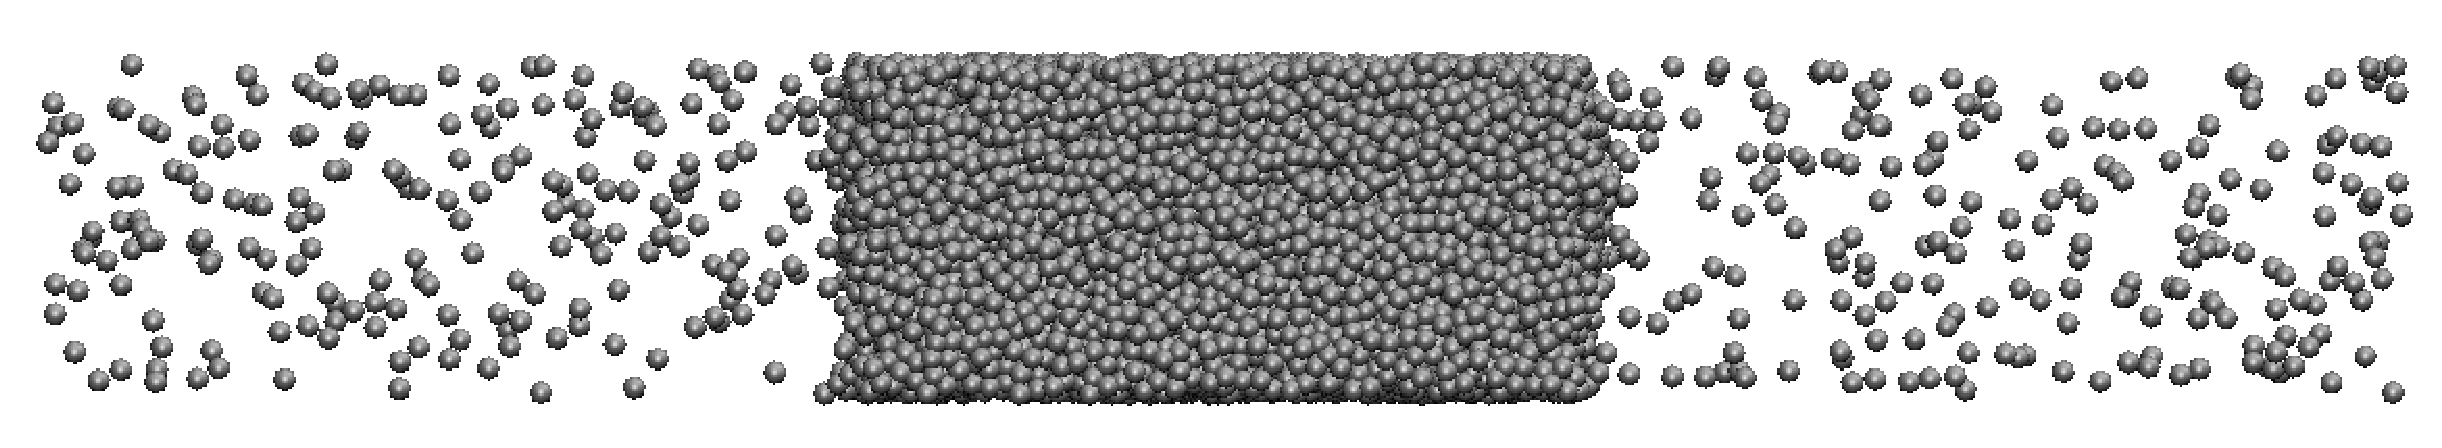
\includegraphics[width=0.9\textwidth]{fig/t0.85-n16000-rc07.5uni/confout.eps}
  \caption{The snapshot of the 16000 Lennard-Jones particle system at
    $T^\ast=0.85$ with a uniform cut-off radius of $r_c^\ast = 7.5$.}
  \label{fig:tmp1}
\end{figure}

Figure \ref{fig:tmp2} presents the real RMS force error (in green
square) in a system using a uniform cut-off raidus of $r_c^\ast =
7.5$. The number density distribution along $x$ direction is shown by
the solid red line for reference.  The error is comparatively constant
at the bulk liquid and gas region. In contrast, two paaks, which are
more than one order of maganitude larger than the force errors in bulk
regions, form at the interfacial region.  The estimated RMS force
error is presented in solid blue line.  The estimate follows the real
error very well at the interfacial region, but slightly over estimate
the error in the bulk regions.  Two components of the force error,
namely the homogeneity error and heterogeneity error are presented in
Fig. \ref{fig:tmp2} by dashed and dotted blue lines, respectively.  In
the bulk regions, the dashed blue line overlaps with the solid blue
line, that means the homogeneity error dominates.  In the interfacial
region, in the contrary, the heterogeneity error dominate, because the
dotted blue line overlaps with the solid one.

\begin{figure}
  \centering
  % 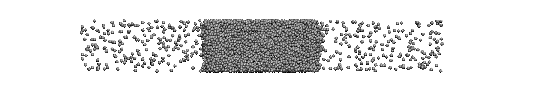
\includegraphics[]{fig/t0.85-n16000-rc07.5uni/confout-02.eps}
  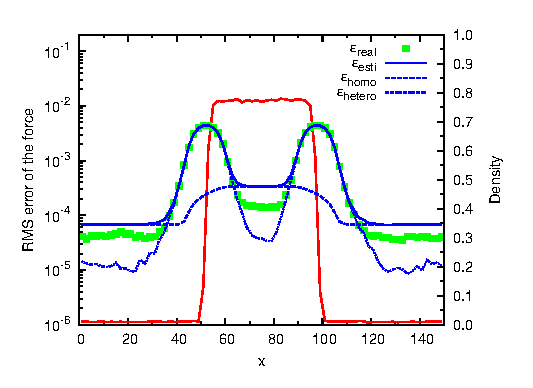
\includegraphics[]{fig/t0.85-n16000-rc07.5uni/error.uniform.eps}
  \caption{The RMS force error distribution of the 16000 Lennard-Jones
    particle system at $T^\ast=0.85$ with a uniform cut-off radius of
    $r_c^\ast = 7.5$. The green squares present the real error. The
    solid blue line is the error estimate by \eqref{eqn:tmp5}. The
    dashed blue line is the homogeneity error contribution, while the
    dotted blue line is the heterogeneity error contribution. The
    density distribution of the system is presented by red solid line
    for reference.  All properties are properly averaged on the $y$
    and $z$ direction, therefore, the profiles are plotted along the
    $x$ direction.  }
  \label{fig:tmp2}
\end{figure}


The Fig. \ref{fig:tmp2} inspires us to develop the adaptive cut-off
method: in the bulk regions, the error is much smaller, therefore, it
is a waste to use the same cut-off radius as the interfacial
regions. As mentioned before, the key idea is to use small cut-off
radius in the bulk regions, so that the RMS force error is uniformly
distributed over the simulation region. In Fig. \ref{fig:tmp3}, we
present the adapted cut-off radius in a solid red line and all errors
in the same notation as the Fig. \ref{fig:tmp2}. The control error
$\mathcal E^\ast_{\textrm{C}} = 0.0045$ is the same as the maximum
error in the uniform cut-off simulation with $r_c^\ast=7.5$. The
cut-off distribution is refined for twice by \eqref{eqn:rc-refine}. In
the interfacial region, the same cut-off radius as the uniform cut-off
simulation, namely $7.5$, is reproduced.  Whereas, in the liquid and
vapor regions, the cut-off radii are $4.75$ and $3.5$, respective,
which is notably reduced. Considering the computational cost grows
with $\mathcal O(r_c^3)$, the adaptive cut-off saves 75 \% and 90 \%
computational cost in the liquid and vapor bulk regions, respectively.
The error is uniformly distributed, except that in the liquid region,
the real error is somewhat lower because the error estimate is not
sharp here. In constrast with the uniform cut-off case,
i.e. Fig. \ref{fig:tmp2}, the error estimate for the vapor region is
very sharp. The same phenominon is observed: the homogeneity error
dominates in the bulk regions, while the heterogeneity error dominates
in the interfacial region.

\begin{figure}
  \centering
  % 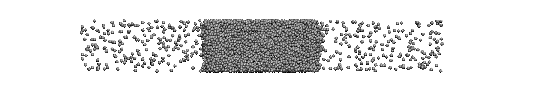
\includegraphics[scale=1]{fig/t0.85-n16000-rc07.5uni/confout-02.eps}
  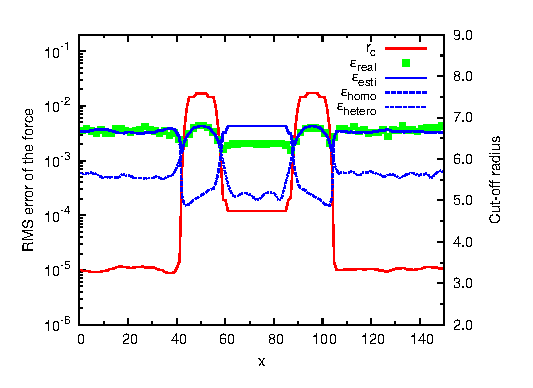
\includegraphics[]{fig/t0.85-n16000-adapt-e0.0045-extend/rcut.and.error.eps}
  \caption{ The RMS force error distribution of the 16000
    Lennard-Jones particle system at $T^\ast=0.85$ with adaptive
    cut-off radius. The control error $\mathcal E^\ast_{\textrm{C}}$
    is the same as the maximum error in the uniform cut-off simulation
    with $r_c^\ast=7.5$.  The resulting cut-off radius distribution is
    presented by the red line. All other notations are the same as
    Fig.~\ref{fig:tmp2}.}
  \label{fig:tmp3}
\end{figure}


In Fig. \ref{fig:tmp4}, we present the mean error force (only $x$
component) by the red solid line. The $y$ and $z$ components of the
mean error force is not shown because their magnitudes are negligible.
On the left interface, the mean error force is along the positive
direction of $x$ axis, namely poiting right.  On the right interface,
the mean error force is of the same maganitude but poiting
left. Therefore, the liquid density should be higher and the vapor
density should be lower than the uniform and adaptive cut-off
simulations.  The real error (in green square) and the homogeneity
error (in blue solid line) are all presented in
Fig. \ref{fig:tmp4}. Clearly the contribution of the heterogeneity
error is successfully removed, because the estimate of homogeneity
error follows the real error perfectly in the interfacial regions.  In
the bulk liquid region, the homogeneity error is slightly
overestimated, which is the same as the uniform and adaptive cut-off
simulations.

\begin{figure}
  \centering
  % 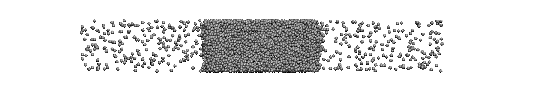
\includegraphics[scale=1]{fig/t0.85-n16000-rc07.5uni/confout-02.eps}
  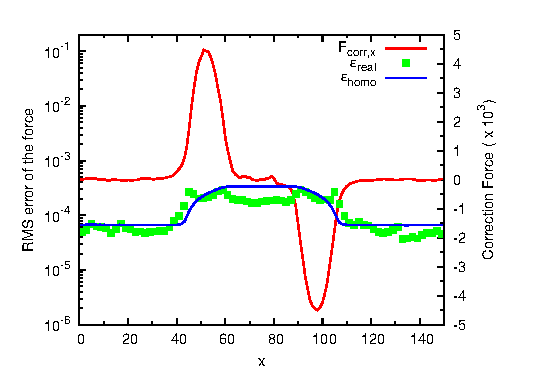
\includegraphics[]{fig/t0.85-n16000-fcorr-rc07.5-feq0200/fcorr.and.error.eps}
  \caption{ The RMS force error distribution of the 16000
    Lennard-Jones particle system at $T^\ast=0.85$ with force
    corrected by the mean error force,
    i.e. eqn. \eqref{eqn:define-fcorr}. The cut-off radius is $r^\ast_c =
    7.5$. The $x$ component of the mean error force is presented by
    the solid red line. The green squares present the real error. The
    solid blue line presents the homogeneity error. }
  \label{fig:tmp4}
\end{figure}


% As mentioned before, form Fig. \ref{fig:tmp2}, the error dominates at
% the interfacial regions. The error estimate is sharp in these
% regions. While in the bulk regions, the error estimate is not sharp,
% but still acceptable. By the adapt cut-off radius MD, the resulting
% distribution (averaged on $y$ and $z$ directions) of cut-off radius is
% given in Fig. \ref{fig:tmp3}. In the interfacial regions, the cut-off
% radius is adapted to $r_c^\ast = 7.5$. In the bulk liquid and vapor
% regions, the cut-off radii are approximatly $5.0$ and $3.5$.  The
% resulting error distribution is ploted in FIg. \ref{fig:tmp4}. It is
% clear that the error is comparatively uniformly distributed in the
% space. The estimate heterogeneity error is also dominant at the
% interfacial region, while the homogeneous error dominants in the bulk
% regions.  Since the computational cost is proportional to $r_c^3$,
% comparing with a simulation using uniform cut-off radius $7.5$, the
% adaptive cut-off simulation saves 3.4 times and 9.8 times
% computational cost, respectively. In total, the adaptive cut-off
% radius method save 50\% of the computational cost.

We test the uniform and adaptive cut-off methods as well as the
correction force method in the mentioned liquid vapor equilibrium
system. The temperatures are controlled to $T^\ast = 0.70,\ 0.85,\
1.10,\ 1.20$ by a Nos\`e-Hoover thermostat. The interested properties are
the liquid-vapor equilibrium density and the surface tension defined
by
\begin{align}
  \gamma = \frac12 \int_{L_x}
  \bigg[\,
  p_x(x) - \frac{p_y(x) + p_z(x)}{2}
  \,\bigg]
  \,\d dx
\end{align}
where $p_x$, $p_y$ and $p_z$ are $x$, $y$ and $z$ component of the
pressure. The convergence of the properties of interest with respect
to the cut-off radius is considered.  For the adaptive cut-off
simulation, the ``cut-off radius'' means the largest cut-off radius
used in the simulation region. 

\begin{figure}
  \centering
  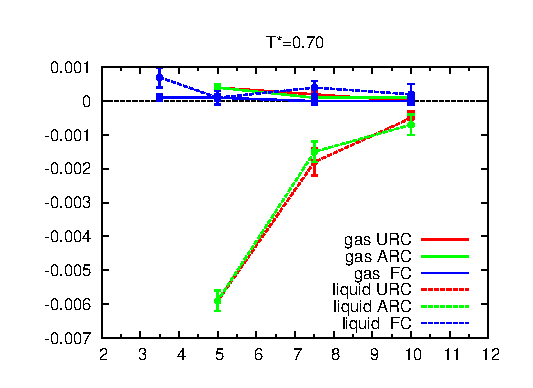
\includegraphics[width=0.49\textwidth]{fig/converge/t0.70.eps} 
  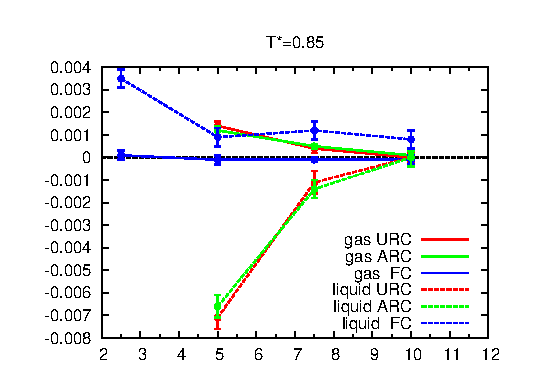
\includegraphics[width=0.49\textwidth]{fig/converge/t0.85.eps} 
  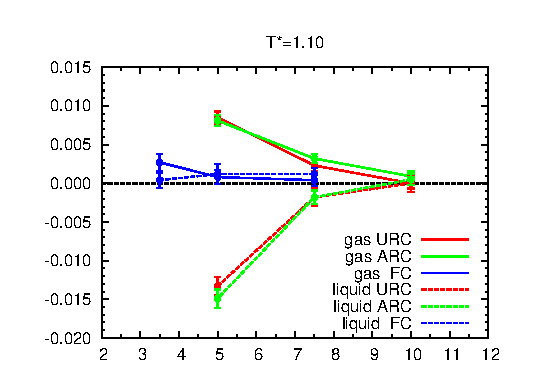
\includegraphics[width=0.49\textwidth]{fig/converge/t1.10.eps} 
  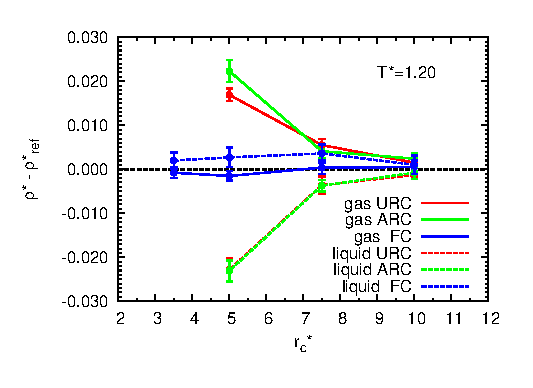
\includegraphics[width=0.49\textwidth]{fig/converge/t1.20.eps} 
  \caption{The convergence of the equilibrium gas and liquid density
    with respect to the cut-off radius. All densities are substracted
    by the reference value, namely, the liquid and vapor density
    meansured with a uniform cut-off radius $r_c^\ast=13$. This figure
    presents the results of three methods, namely the uniform cut-off
    (URC), the adaptive cut-off (ARC) and the force correction (FC)
    method. }
  \label{fig:tmp5}
\end{figure}

In the Fig. \ref{fig:tmp5}, the convergence of the equilibrium density
is investigated. The red, green and blue points presents the results
of uniform, adaptive and force correction simulations, respectively.
The gas densities are connected by the solid lines, and the liquid
densities are connected by the dashed lines for clarity. All data are
substracted by the reference results, which are calculated by uniform
cut-off simulations with a cut-off radius $r_c^\ast=13$.  In the
higher temperature cases, the thermodynamic flucuation of the system
is stronger. Therefore, the meansurement of densities are less
accurate in higher temperature cases than in lower temperature cases.
At $T^\ast = 0.70$, the gas density is more accurate than the liquid
density, while at $T^\ast = 1.20$, the gas and liquid densities are of
the same accuracy.

The liquid and gas densities of the uniform and the adaptive cut-off
methods are almost identical using the same cut-off radius. This
observation is also true for the surface tension, see
Fig. \ref{fig:tmp6}. This indicates that controlling the maximum of
force error (see Tab. \ref{tab:tmp1}) and introducing larger
homogeneous force error in the bulk liquid/gas regions will not
disturb the accuracy of equilibrium densities and surface tension.
The adaptive cut-off method roughly saves one half of the
computational cost (see Tab. \ref{tab:tmp1}). The benefit of the
adaptive cut-off depends on the system geometry: if the work load
mainly concentrates on the bulk phase region, the adaptive cut-off
will save a lot computational expense. On the other hand, if the
interfacial region is computationally intensive, the adaptive will not
improve the efficency greatly.

The force correction method presents a perfect convergence when the
cut-off radius is equal to or larger than 5, and the result at a
cut-off as small as 3.5 is acceptable. Comparing the results of force
correction method at $r_c^\ast = 3.5$ and uniform cut-off radius
method at $r_c = 7.5$, the maximum force error of the former method is
3--5 times larger than the later (see Tab. \ref{tab:tmp1}), however,
the measure of equilibrium densities and surface tension are
comparable to and sometimes even better than the later (see
Fig. \ref{fig:tmp5} and \ref{fig:tmp6}). In the force correction
simulation, the heterogeneity error is screened out and the force
error term is dominated by the homogeneity error. And in the uniform
cut-off simulation the force error is dominated by the heterogeneity
error in the interfacial regions. Therefore, the homogeneity error and
heterogeneity error play different roles in the simulations.  The
heterogeneity error stems from the non-vanishing value of the mean
error force, which is alway pointing at one certain direction (the
same direction as the low-to-high density jump), see
Fig. \ref{fig:tmp4} for example. The homogeneity error is actually the
variation of the corrected error force that may be cancelled by itself
in a long time. The reason is the corrected error force has a
varnished mean value (see eqn. \eqref{eqn:mean-fcorr}), so it may
point to any direction with the same possibility.  With the same
cut-off radius, the computational cost of the force correction and
uniform cut-off methods are nearly the same, see
Tab. \ref{tab:tmp1}. However, the maximum force error of the force
correction method is about one order of maganitude more precise,
comparing with the uniform cut-off simulations.

\begin{figure}
  \centering
  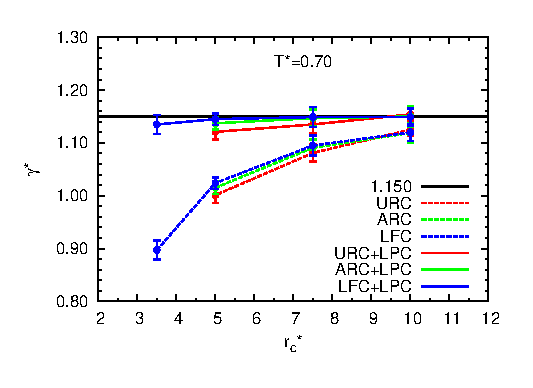
\includegraphics[width=0.49\textwidth]{fig/converge/tension.t0.70.eps} 
  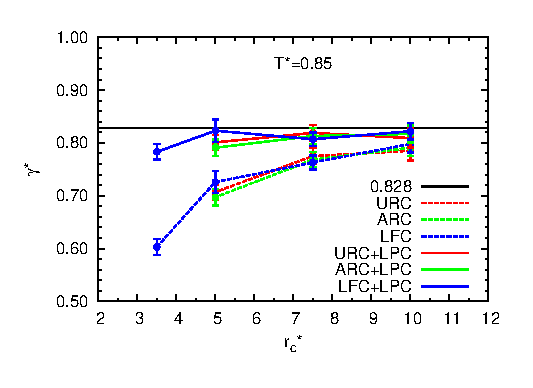
\includegraphics[width=0.49\textwidth]{fig/converge/tension.t0.85.eps} 
  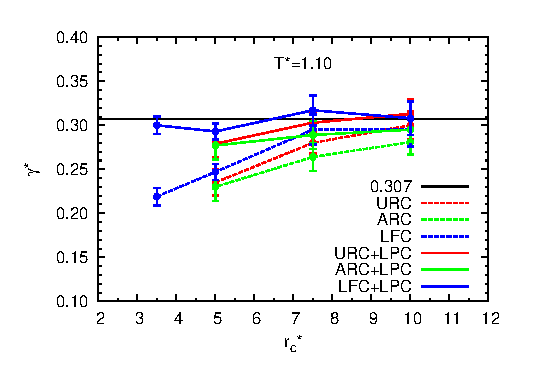
\includegraphics[width=0.49\textwidth]{fig/converge/tension.t1.10.eps} 
  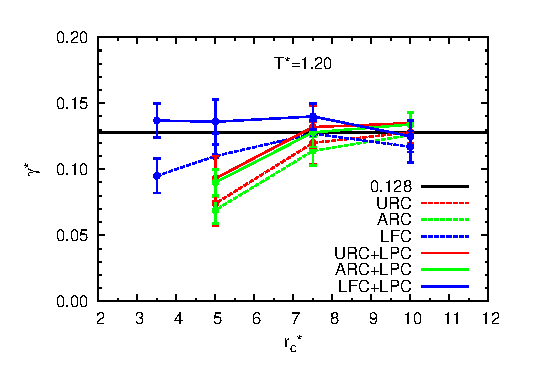
\includegraphics[width=0.49\textwidth]{fig/converge/tension.t1.20.eps} 
  \caption{The convergence of the surface tension with respect to the
    cut-off radius.  This figure presents the results of three
    methods, namely the uniform cut-off (URC), the adaptive cut-off
    (ARC) and the force correction (FC) method.  The results with and
    without heterogeneous pressure correction (HPC) are shown together
    for comparison. The reference surface tensions, shown by solid
    black lines, are measured by the uniform cut-off method with
    $r_c^\ast=13$ using HPC.}
  \label{fig:tmp6}
\end{figure}

The convergence of the surface tension with respect to the cut-off
radius is shown in the Fig. \ref{fig:tmp6}. The color notation is the
same as Fig. \ref{fig:tmp5}.  Surface tensions measured with and
without heterogeneous pressure correction are connected by solid and
dashed lines, respectively.  The reference surface tension is
presented by the black solid lines. The heterogeneous pressure
correction improve the surface tention measurement greatly. The
discrepancy between the corrected and uncorrected pressure is the
value of the correction, which decreases with increasing cut-off
radius. However, even at $r_c^\ast=10$, the correction is not
negligible for $T^\ast = 0.70$ and $T^\ast = 0.85$. At higher
temperature, the statistical uncertainty gets larger, and better
convergence is achieved at small cut-off radius.

% Although the force correction is a
% little better, no substential difference between the different
% simulation methods is observed. However, the With the
% pressure correction, the result is acceptable at cut-off 5.0 and
% satisfactorily converged at cut-off 7.5.

\begin{table}
  \centering
  \caption{
    The maximum RMS force error and computational cost of 
    of three methods, namely the uniform cut-off
    (URC), the adaptive cut-off (ARC) and the force correction (FC) method.
    The computational cost is the number of pairwise interaction 
    measurements performed by the program, which should be mashine-independent.
  }\label{tab:tmp1}
  \begin{tabular*}{0.50\textwidth}{c|c|@{\extracolsep{\fill}}ccc}\hline\hline
    $T^\ast$ &$r^\ast_{c}$ & \textrm{method} & $\max\mathcal E^\ast$ & Cost($\times 10^{-6}$) \\ \hline
    & 3.5 &\textrm{FC } & $1.4\times 10^{-2}$ & 3.4 \\\cline{2-5}
    &     &\textrm{URC} & $2.5\times 10^{-2}$ & 7.9 \\
    & 5.0 &\textrm{ARC} & $2.4\times 10^{-2}$ & 4.6 \\
    &     &\textrm{FC } & $2.0\times 10^{-3}$ & 8.8 \\\cline{2-5}
    &     &\textrm{URC} & $4.9\times 10^{-3}$ & 27 \\
0.70& 7.5 &\textrm{ARC} & $4.9\times 10^{-3}$ & 13 \\
    &     &\textrm{FC } & $2.5\times 10^{-4}$ & 27 \\\cline{2-5}
    &     &\textrm{URC} & $1.6\times 10^{-3}$ & 59 \\
    &10.0 &\textrm{ARC} & $1.6\times 10^{-3}$ & 29 \\
    &     &\textrm{FC } & $5.8\times 10^{-5}$ & 59 \\ \hline\hline
    & 3.5 &\textrm{FC } & $1.4\times 10^{-2}$ & 3.1 \\\cline{2-5}
    &     &\textrm{URC} & $2.1\times 10^{-2}$ & 7.1 \\
    & 5.0 &\textrm{ARC} & $1.8\times 10^{-2}$ & 4.6 \\
    &     &\textrm{FC } & $1.9\times 10^{-3}$ & 7.9 \\\cline{2-5}
    &     &\textrm{URC} & $4.4\times 10^{-3}$ & 24 \\
0.85& 7.5 &\textrm{ARC} & $4.3\times 10^{-3}$ & 12 \\
    &     &\textrm{FC } & $3.0\times 10^{-4}$ & 24 \\\cline{2-5}
    &     &\textrm{URC} & $1.4\times 10^{-3}$ & 53 \\
    &10.0 &\textrm{ARC} & $1.4\times 10^{-3}$ & 26 \\
    &     &\textrm{FC } & $5.3\times 10^{-5}$ & 53 \\ \hline\hline
  \end{tabular*}
  \begin{tabular*}{0.49\textwidth}{c|c|@{\extracolsep{\fill}}ccc}\hline\hline
    $T^\ast$ &$r^\ast_{c}$ & \textrm{method} & $\max\mathcal E^\ast$ & Cost($\times 10^{-6}$) \\ \hline
    & 3.5 &\textrm{FC } & $1.3\times 10^{-2}$ & 3.8 \\\cline{2-5}
    &     &\textrm{URC} & $1.5\times 10^{-2}$ & 5.6 \\
    & 5.0 &\textrm{ARC} & $1.5\times 10^{-2}$ & 3.2 \\
    &     &\textrm{FC } & $1.7\times 10^{-3}$ & 9.9 \\\cline{2-5}
    &     &\textrm{URC} & $3.3\times 10^{-3}$ & 17 \\
1.10& 7.5 &\textrm{ARC} & $3.5\times 10^{-3}$ & 8.8 \\
    &     &\textrm{FC } & $1.8\times 10^{-4}$ & 18 \\\cline{2-5}
    &     &\textrm{URC} & $1.1\times 10^{-3}$ & 39 \\
    &10.0 &\textrm{ARC} & $1.0\times 10^{-3}$ & 19 \\
    &     &\textrm{FC } & $4.2\times 10^{-5}$ & 39 \\ \hline\hline
    & 3.5 &\textrm{FC } & $1.2\times 10^{-2}$ & 1.8 \\\cline{2-5}
    &     &\textrm{URC} & $1.1\times 10^{-2}$ & 4.2 \\
    & 5.0 &\textrm{ARC} & $9.2\times 10^{-3}$ & 2.9 \\
    &     &\textrm{FC } & $1.5\times 10^{-3}$ & 4.6 \\\cline{2-5}
    &     &\textrm{URC} & $2.5\times 10^{-3}$ & 14 \\
1.20& 7.5 &\textrm{ARC} & $2.4\times 10^{-3}$ & 7.7 \\
    &     &\textrm{FC } & $1.5\times 10^{-4}$ & 14 \\\cline{2-5}
    &     &\textrm{URC} & $8.2\times 10^{-4}$ & 30 \\
    &10.0 &\textrm{ARC} & $8.3\times 10^{-4}$ & 17 \\
    &     &\textrm{FC } & $3.3\times 10^{-5}$ & 31 \\\hline\hline
  \end{tabular*}
\end{table}



% The equilibrium liquid and vapor densities with respect to
% the cut-off radius are presented in Fig. \ref{fig:tmp5}. For the
% adaptive cut-off simulation, the data points represent the largest
% cut-off radius used in the simulations. All the results are
% substracted by the reference results, which are calculated at uniform
% cut-off radius of 13, for a clear comparison. Solid and dashed lines
% are added to the data points of vapor and liquid densities
% respectively. For the uniform and adaptive cut-off simulations, the
% cut-off radii 5, 7.5 and 10 are considered. For the force correction,
% the cut-off 3.5 is investigated in addition. We perform simulations at
% different temperature: that are denoted in the plots.





% \begin{figure}
%   \centering
%   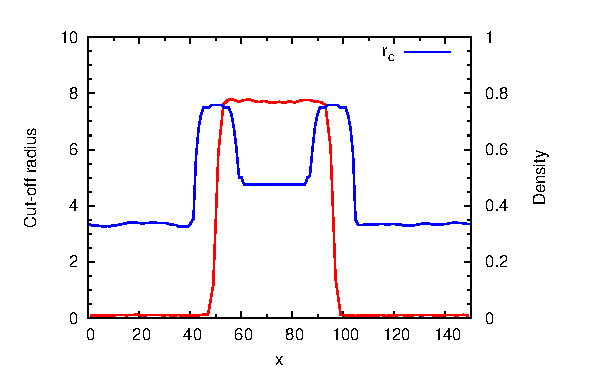
\includegraphics[]{fig/t0.85-n16000-adapt-e0.0045-extend/rcut.adapt.eps}
%   \caption{The adapted cut-off radius of the 16000 Lennard-Jones
%     particle system at $T^\ast=0.85$.}
%   \label{fig:tmp3}
% \end{figure}


% \begin{figure}
%   \centering
%   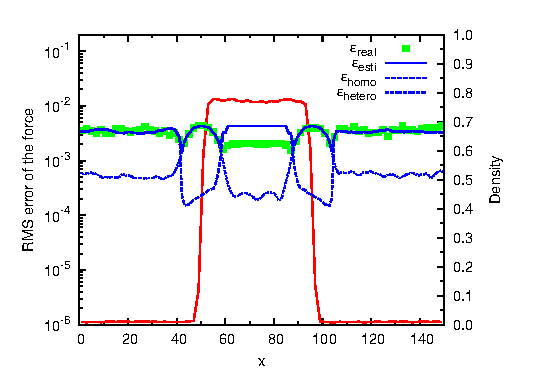
\includegraphics[]{fig/t0.85-n16000-adapt-e0.0045-extend/error.adapt.eps}
%   \caption{The error distribution of the adaptive-cut-off 16000
%     Lennard-Jones particle system at $T^\ast=0.85$.}
%   \label{fig:tmp4}
% \end{figure}


% \begin{figure}
%   \centering
%   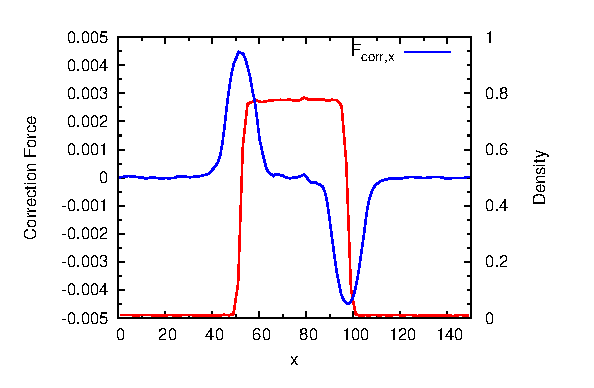
\includegraphics[]{fig/t0.85-n16000-fcorr-rc07.5-feq0200/fcorr.eps}
%   \caption{The correction force simulation of the 16000 Lennard-Jones
%     particle system at $T^\ast=0.85$.}
%   \label{fig:tmp3}
% \end{figure}


% \begin{figure}
%   \centering
%   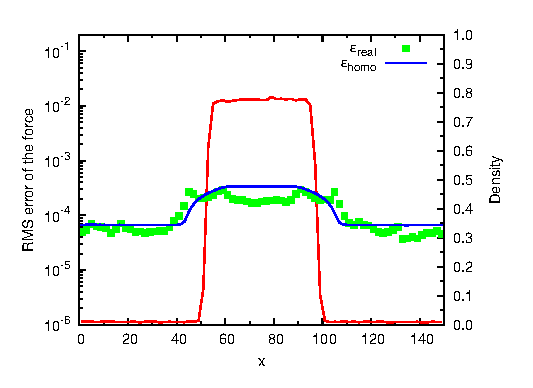
\includegraphics[]{fig/t0.85-n16000-fcorr-rc07.5-feq0200/error.fcorr.eps}
%   \caption{The correction force simulation of the adaptive-cut-off 16000
%     Lennard-Jones particle system at $T^\ast=0.85$.}
%   \label{fig:tmp4}
% \end{figure}








\subsection{Collision of nanoscale Lennard-Jones clusters}
\label{sec:tmp2.2}

In this section, we test the adaptive cut-off method and the force
correction method in a dynamical problem: collision of nanoscale
Lennard-Jones clusters. Two initial Lennard-Jones clusters, denoted by
$A$ and $B$, are setup in the simulation box, each of which contains
the same number of particles $N_A = N_B = 10792$, with a diameter of
$d^\ast\approx 27$. The initial velocity of the clusters are $\v u_A =
\frac12(u, 0, 0)$ and $\v u_B = -\frac12(u, 0, 0)$, see
Fig. \ref{fig:tmp7}. The impact parameter $D$ is defined by the $z$
corrdinate difference between the center of mass (COM) of the
clusters. The unitless impact factor defined by
\begin{align}
  x = \frac D d
\end{align}
is used to measure how far off-center the collision happens. If $x =
0$ the collision is head-on, while $x=1$ the collision is avoided.
Ref. \cite{kalweit2006collision} investigated a board range
combination of velocity $u$ and impact factor $x$, and identified
three major collision modes: the coalescence, the streching seperation
and the shattering. The major modes were further classified into a
series submodes. In this paper, we want to study the how the collision
properties of interests are affected by the force calculation
precision, therefore, we will NOT investigate a broad range of
parameters, but focus on one special case: $u^\ast = 2.2$ and $x =
0.6$, where poor precision of force calculation will lead to wrong
major collision modes.

\begin{figure}
  \centering
  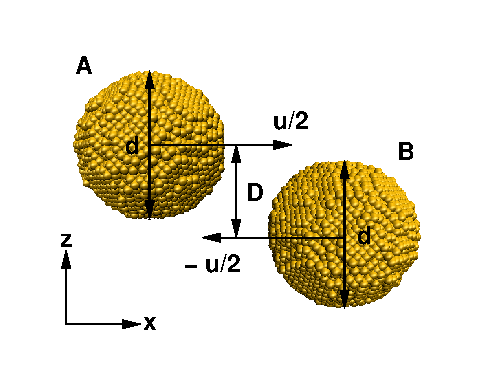
\includegraphics[]{fig/collision-init/init.2.eps}
  \caption{The initial setup of cluster $A$ and $B$. The initial
    velocity are equal in maganitude but on opposite direction.}
  \label{fig:tmp7}
\end{figure}

In Fig. \ref{fig:tmp8} and \ref{fig:tmp9}, we present the trajectory
of cluster $A$ and COM distance between the two clusters,
respectively. Three different cut-off radii of uniform cut-off
simulation are considered. In this case the two clusters collide and
form one rotating cluster. It is obvious that the trajectory of
$r_c^\ast = 2.5$ is completely wrong: two clusters seperate after
collision. The $r_c^\ast = 5.0$ trajectory is reasonably good, but the
COM distance converges only when $r_c^\ast = 7.5$. This means the
precision of force calculation is crucial in the study of collision
dynamics. Althougth the precision of the adaptive cut-off method of
$r_c^\ast = 5$ is the as uniform cut-off $r_c^\ast = 5$, the former
produce better trajectory than the later. The force correction method
that get rid of the heterogeneity error produces correct trajectory,
but the motion along the trajectory is somewhat faster than other
methods (see also the angular velocity in Fig. \ref{fig:tmp11}).

\begin{figure}
  \centering
  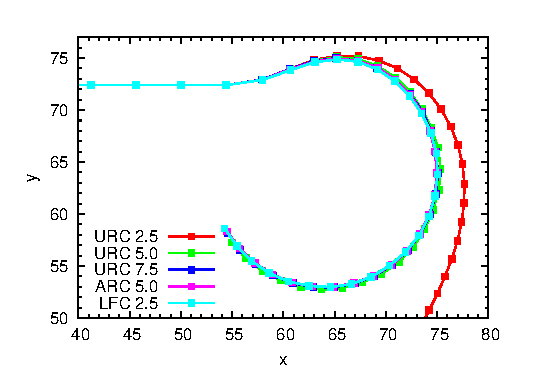
\includegraphics[]{fig/trajs.eps}
  \caption{The center of mass trajectory of cluster A. Uniform cut-off
    $r_c^\ast = 2.5,\ 5.0,\ 7.5$, adaptive cut-off $r_c = 5.0$ and
    force correction of $r^\ast_c = 2.5$ are investigated.  The time
    interval between two neighboring squares on the trajectory is 4.
  }
  \label{fig:tmp8}
\end{figure}

\begin{figure}
  \centering
  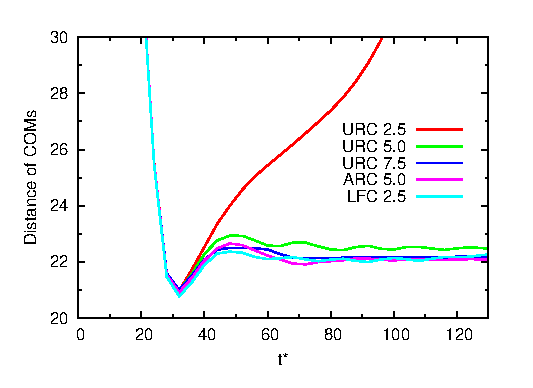
\includegraphics[width=0.49\textwidth]{fig/dists.eps}
  \caption{The distance between the center of mass of cluster $A$ and
    cluster $B$ as a function of time.}
  \label{fig:tmp9}
\end{figure}


The RMS force error of $r_c^\ast = 5.0$ uniform cut-off simulation,
the cut-off distribution of adaptive cut-off method and the magnitude
of the mean error force are plotted in Fig. \ref{fig:tmp8}.  The
configuration of the two clusters (colored in gray and yellow) are
presented on the top for reference. The same as the liquid-vapor
equilibrium simulation, the force error located at the interfacial
region, namely the boundary of the clusters. Inside and outside the
clusters, the error is much lower.  The maximum cut-off used in the
adaptive cut-off simulation is 5.0, which follows the large error
region perfectly. The large cut-off region is much border than the
large error region, because it is refined by twice to keep track of
the possible moving of the clusters.  The mean error force also
follows the boundary of the colliding clusters. In the bulk region
of the clusters, the correction force is neglectable.

\begin{figure}
  \centering
  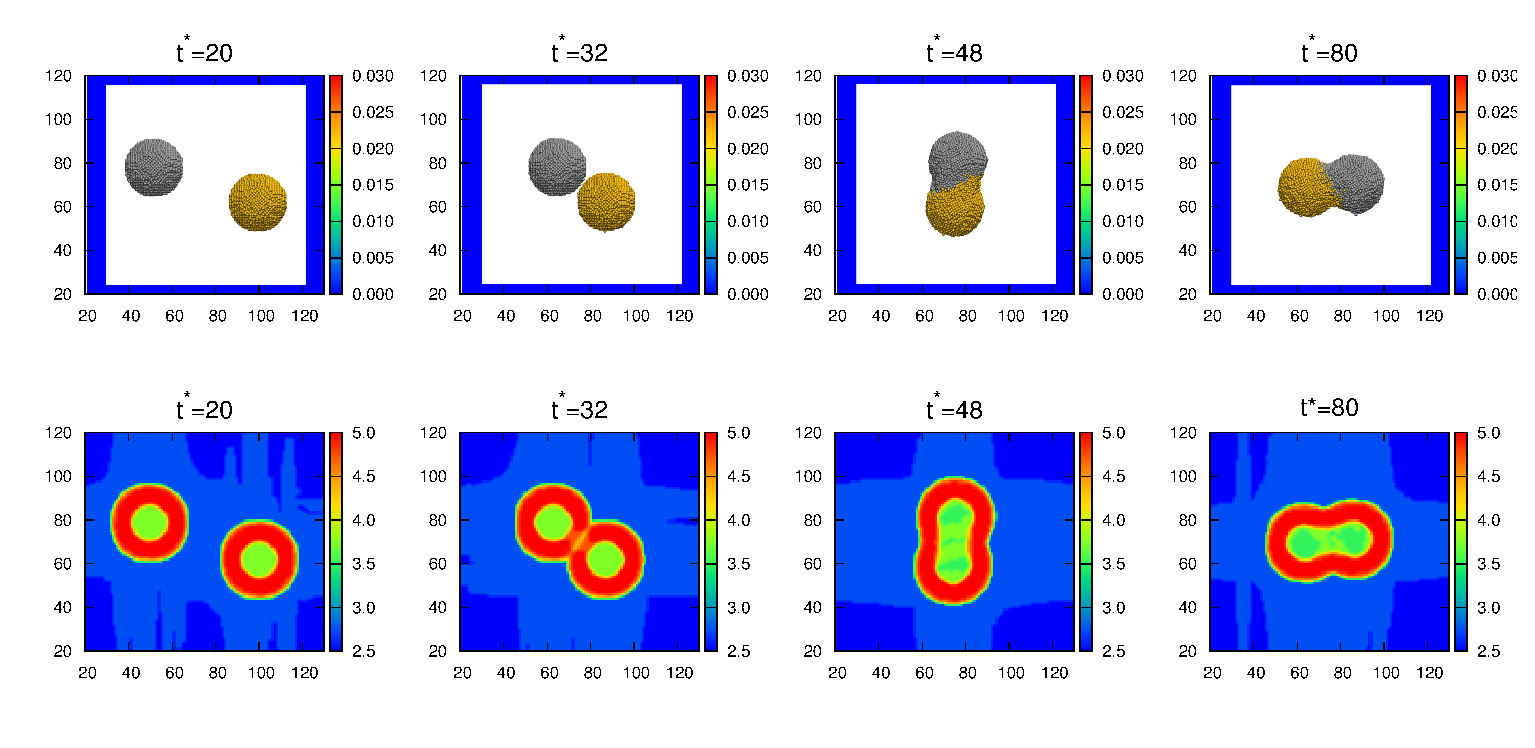
\includegraphics[width=0.90\textwidth]{fig/error-rcut-ball.eps} 
  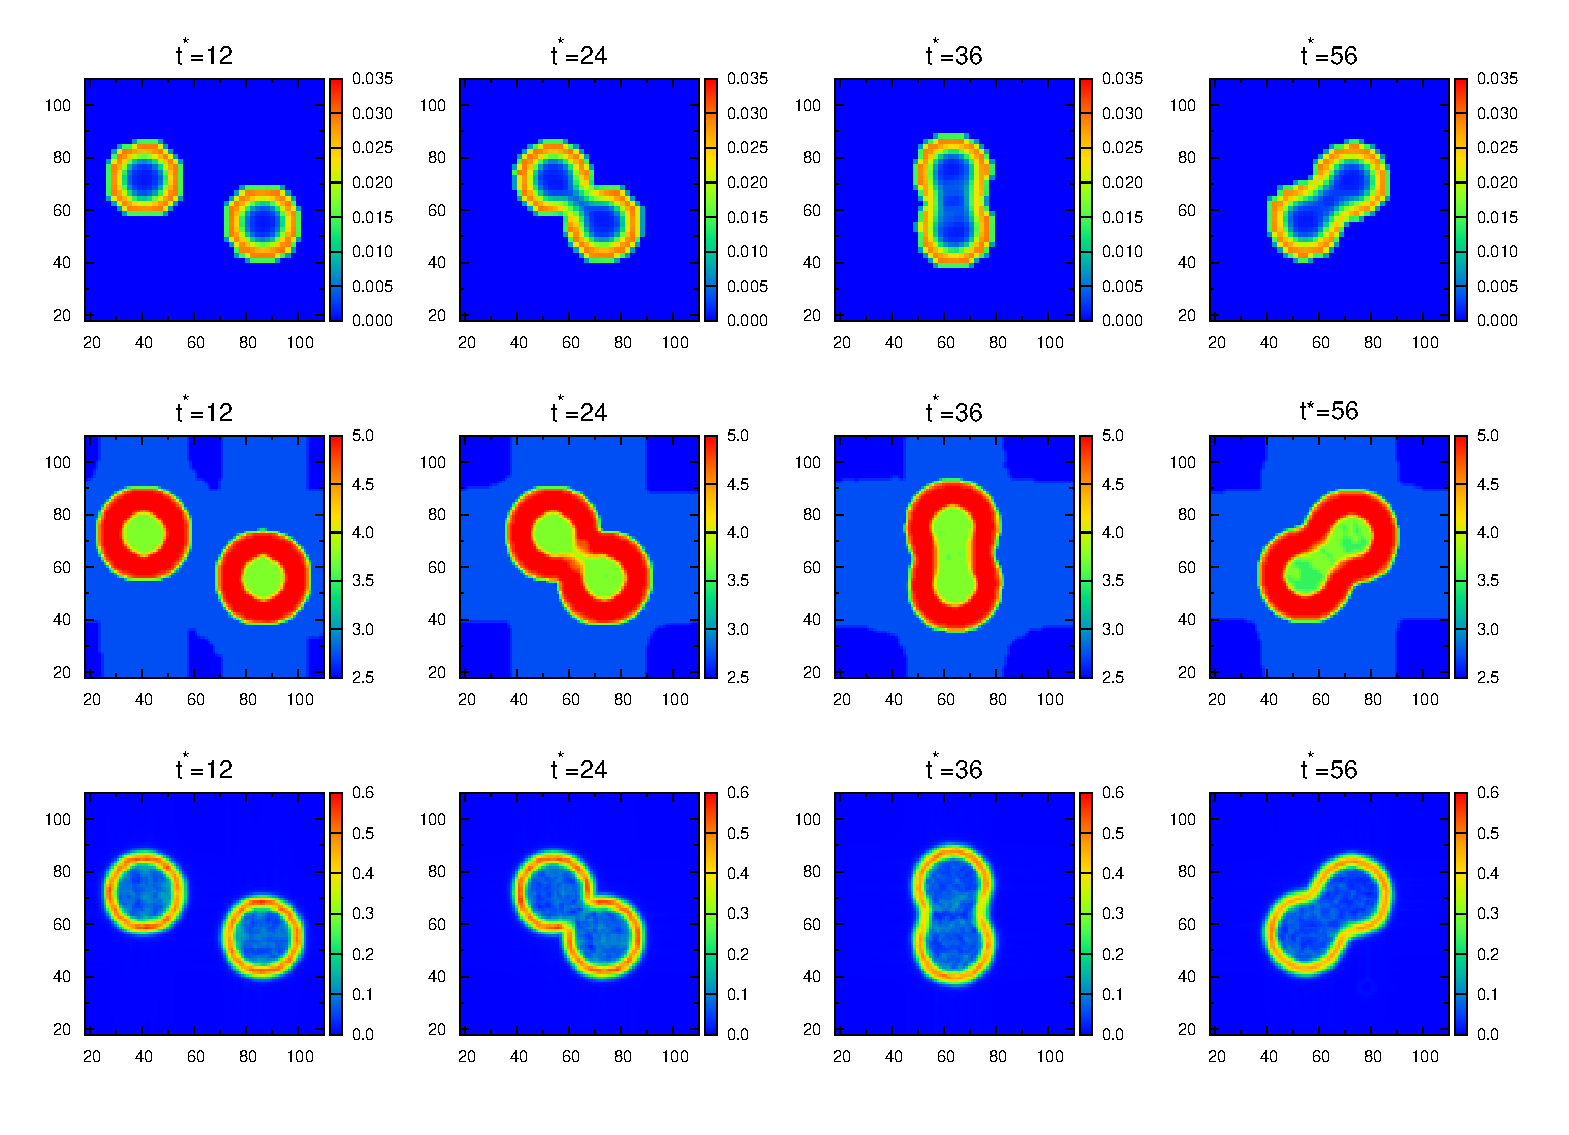
\includegraphics[width=0.90\textwidth]{fig/error-rcut.eps}
  \caption{normal words}
  \label{fig:tmp10}
\end{figure}


The angular velocity is presented in Fig. \ref{fig:tmp11}. The force
correction result is not as precise as other simulations excluding
uniform $r_c = 2.5$ simulation.  The value of the mean error force is
updated every \recheck{aaa} time steps, so considering the moving of the clusters,
it is not the up-to-date value.
% This because the correction force is
% not precise because it is calculated every \recheck{aaa} steps.
In the Fig. \ref{fig:tmp12}, the angular moment, which should be
preserved is presented. All uniform simulations preserved the angular
moment perfectly. The angular moment of the adaptive cut-off
simulation, which does not precisly preserve the Newton's third law,
shows deviation but is still around the correct value. However, the
angular moment of the force correction simulation flies away from the
the correct value by 1 \% at $t^\ast = 130$.

\begin{figure}
  \centering
  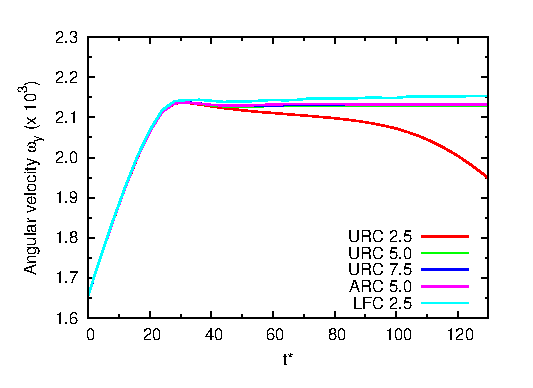
\includegraphics[width=0.49\textwidth]{fig/wy.eps}
  \caption{normal words}
  \label{fig:tmp11}
\end{figure}

\begin{figure}
  \centering
  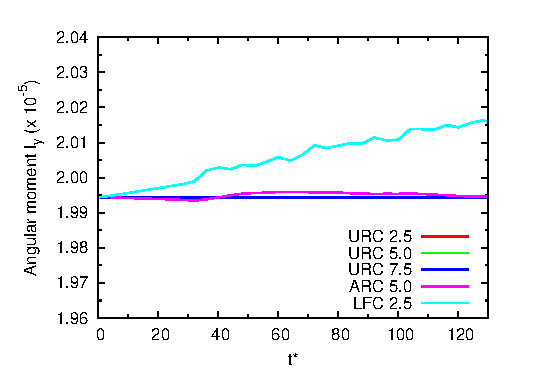
\includegraphics[width=0.49\textwidth]{fig/ly.eps}
  \caption{normal words}
  \label{fig:tmp12}
\end{figure}



\section{Conclusion}\label{sec:conclusion}


% \newpage

\bibliography{ref}{}
\bibliographystyle{unsrt}


\end{document}
